% Composition 2 — Diamond
% El Gólem, 2026-05-23
%
% The inscription's diamond geometry — root, N strands, join — rendered
% as a Kandinsky composition. Overlapping color discs at each topological
% position; thin black lines tracing the transaction graph; floating text
% naming the structural roles. Less literal than Composition I; the
% diamond is half-visible underneath the abstraction.
\documentclass[tikz,border=4mm]{standalone}
\usepackage[T1]{fontenc}
\usepackage{xcolor}
\definecolor{kr}{HTML}{c83727}
\definecolor{ky}{HTML}{e8b73a}
\definecolor{kb}{HTML}{2b62a8}
\definecolor{kg}{HTML}{2a7a4d}
\definecolor{kp}{HTML}{6e3a8a}    % deep violet
\definecolor{kw}{HTML}{f4ead8}
\definecolor{ki}{HTML}{1a1a1a}
\definecolor{kgold}{HTML}{c2a76b}
\begin{document}
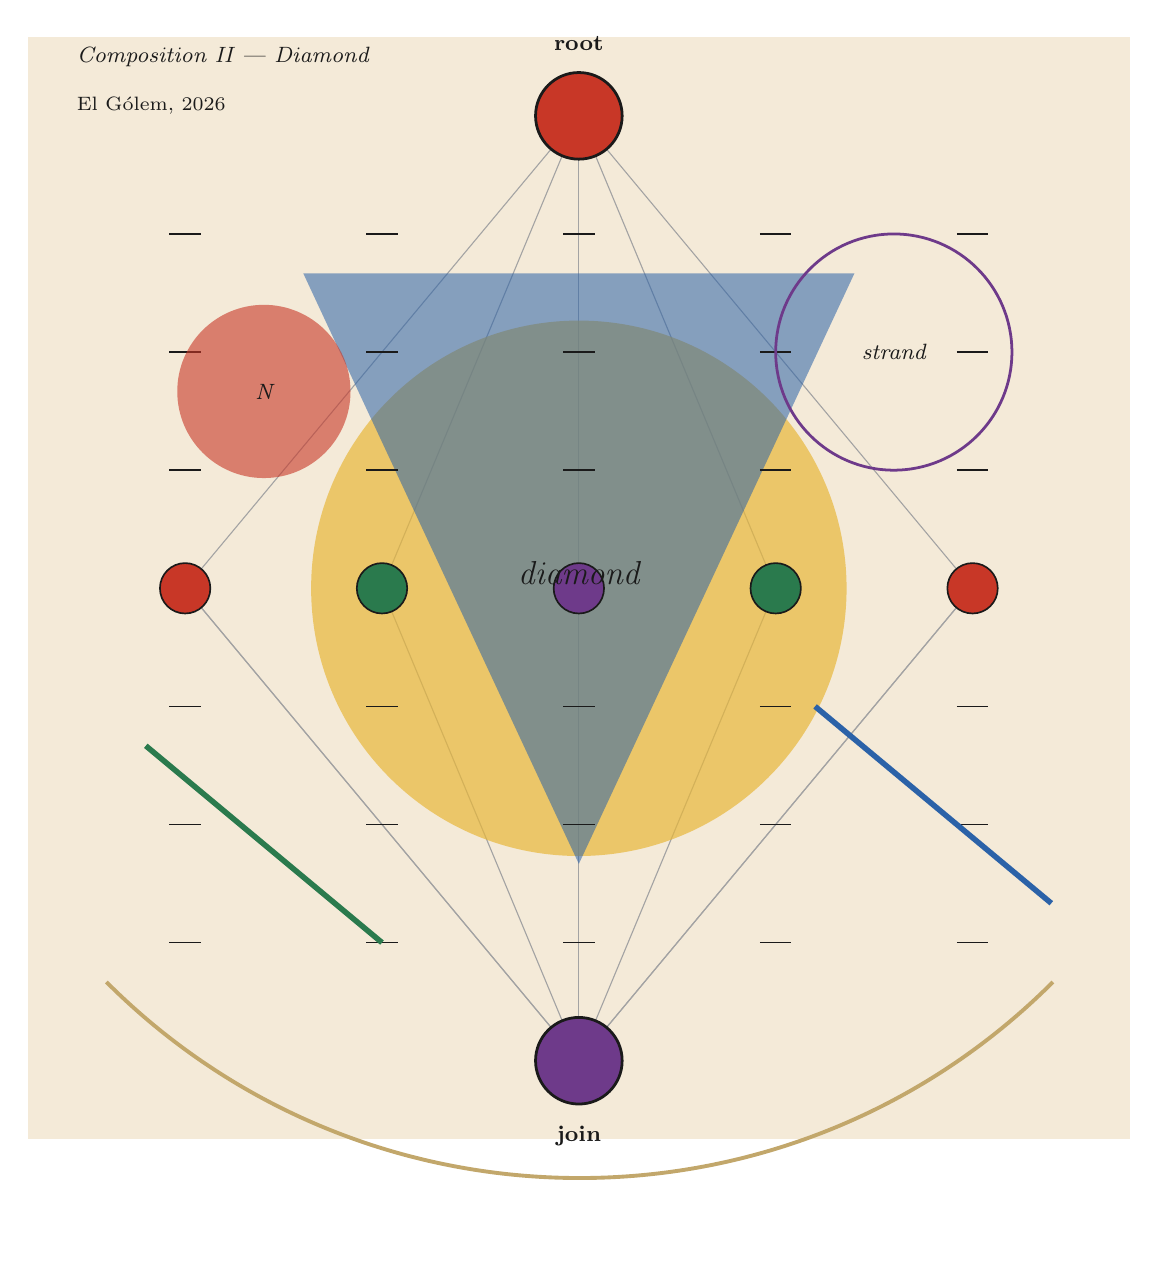
\begin{tikzpicture}[x=1cm,y=1cm]
  \fill[kw] (-7,-7) rectangle (7,7);

  % The underlying diamond skeleton (faint)
  \draw[ki!40,line width=0.4pt] (0,6) -- (-5,0) -- (0,-6) -- (5,0) -- cycle;
  \draw[ki!40,line width=0.4pt] (0,6) -- (-2.5,0);
  \draw[ki!40,line width=0.4pt] (0,6) -- (0,0);
  \draw[ki!40,line width=0.4pt] (0,6) -- (2.5,0);
  \draw[ki!40,line width=0.4pt] (-5,0) -- (0,-6);
  \draw[ki!40,line width=0.4pt] (-2.5,0) -- (0,-6);
  \draw[ki!40,line width=0.4pt] (0,0) -- (0,-6);
  \draw[ki!40,line width=0.4pt] (2.5,0) -- (0,-6);
  \draw[ki!40,line width=0.4pt] (5,0) -- (0,-6);

  % Large yellow disc — the central act
  \fill[ky,opacity=0.7] (0,0) circle (3.4);

  % Blue triangle (downward) — gravity, descent, the closing of the diamond
  \fill[kb,opacity=0.55] (-3.5,4) -- (3.5,4) -- (0,-3.5) -- cycle;

  % Red disc top — the root
  \fill[kr] (0,6) circle (0.55);
  \draw[ki,line width=1pt] (0,6) circle (0.55);
  \node[ki,font=\bfseries\footnotesize,anchor=south] at (0,6.7) {root};

  % Strand seeds (5 small discs along the middle horizontal)
  \foreach \x/\c in {-5/kr, -2.5/kg, 0/kp, 2.5/kg, 5/kr} {
    \fill[\c] (\x,0) circle (0.32);
    \draw[ki,line width=0.6pt] (\x,0) circle (0.32);
  }

  % Join — purple disc at the bottom
  \fill[kp] (0,-6) circle (0.55);
  \draw[ki,line width=1pt] (0,-6) circle (0.55);
  \node[ki,font=\bfseries\footnotesize,anchor=north] at (0,-6.7) {join};

  % Knot marks along each strand (small horizontal dashes)
  \foreach \x in {-5,-2.5,0,2.5,5} {
    \foreach \y in {-4.5,-3,-1.5,1.5,3,4.5} {
      \draw[ki,line width=0.5pt] (\x-0.2,\y) -- (\x+0.2,\y);
    }
  }

  % Floating geometric elements — Kandinsky vocabulary
  \draw[kp,line width=1pt] (4,3) circle (1.5);
  \fill[kr,opacity=0.6] (-4,2.5) circle (1.1);
  \draw[kg,line width=2pt] (-5.5,-2) -- (-2.5,-4.5);
  \draw[kb,line width=2pt] (3,-1.5) -- (6,-4);

  % Bordado-gold rule arc — a partial frame
  \draw[kgold,line width=1.4pt] (-6,-5) arc (-135:-45:8.5);

  % Floating typography
  \node[ki,font=\itshape] at (0,0.2) {\large diamond};
  \node[ki,font=\itshape\footnotesize] at (-4,2.5) {N};
  \node[ki,font=\itshape\footnotesize] at (4,3) {strand};

  % Annotation
  \node[ki,font=\itshape\footnotesize,anchor=south west] at (-6.5,6.5) {Composition II --- Diamond};
  \node[ki,font=\scriptsize,anchor=south west] at (-6.5,5.9) {El G\'olem, 2026};
\end{tikzpicture}
\end{document}
